\documentclass{article}
\usepackage[T1]{fontenc}
\usepackage{lmodern}
\usepackage{graphicx}
\usepackage{amsmath,amssymb}
\usepackage[a4paper,margin=2cm]{geometry}
\usepackage[absolute,overlay]{textpos}
\setlength{\TPHorizModule}{1mm}
\setlength{\TPVertModule}{1mm}
\usepackage[indonesian]{babel}
\usepackage{hyperref}
\setlength{\emergencystretch}{2em}
% unit: Halaman 25

\begin{document}

% === Halaman 25 (python/native) ===

Steganografi Digital

• Steganografi digital: penyembunyian pesan digital di dalam dokumen digital 

lainnya. 

• Carrier file: dokumen digital yang digunakan sebagai media untuk 

menyembunyikan pesan. 

25

1. Teks

   “Kita semua bersaudara”

2. Audio 


3. Gambar (image)

4. Video 


- bmp

- jpeg

- gif

- png

- wav

- mp3

-Txt

- doc

- html

-mpeg

- avi

- mp4

% deskripsi: gambar native xref 142
\noindent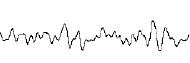
\includegraphics[width=0.85\textwidth]{../../images/python/page_025_img_01.png}

% deskripsi: gambar native xref 145
\noindent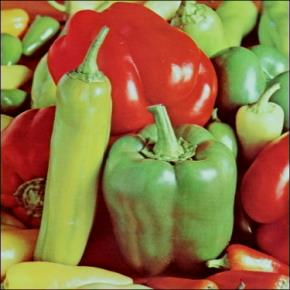
\includegraphics[width=0.85\textwidth]{../../images/python/page_025_img_02.jpeg}

% deskripsi: gambar native xref 146
\noindent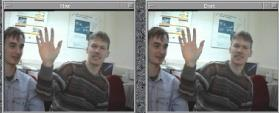
\includegraphics[width=0.85\textwidth]{../../images/python/page_025_img_03.jpeg}

\end{document}
